\documentclass[12pt]{ai_conquer2026}
\addbibresource{references.bib}

\title{%
  \begin{center}
        \Large {AI VIET NAM -- AI Conquer 2026}\\[.5ex]  
        \Huge \textbf{Guidance to AI Conquer 2026 \\ 
        (\LaTeX\space Template)}\\[.5ex]
  \end{center}
}

% Author --------------------------------------------------------------------
\posttitle{
    \author{
        \begin{minipage}{\textwidth}
        \centering
        {
        \vspace{-1.5em}
          Ban biên soạn AIO
        }\\
      \end{minipage}
    }
}
% \setlength{\drop}{-8em}
\date{}

% Header --------------------------------------------------------------------
\pagestyle{fancy}
\fancyhf{}
\lhead{\href{https://www.facebook.com/aivietnam.edu.vn}{\textcolor{aivnGreen}{\bfseries AI VIET NAM (AI Conquer 2026)}}}
\rhead{\href{https://aivietnam.edu.vn/}{\textcolor{aivnGreen}{\bfseries aivietnam.edu.vn}}}
\fancyfoot[C]{\thepage}
\renewcommand{\headrulewidth}{1.0pt}
\renewcommand{\headrule}{{\color{aivnGreen}\hrule width\headwidth height\headrulewidth \vskip-\headrulewidth}}


\begin{document}
\maketitle
\vspace{-5.5em}
\setlength{\epigraphwidth}{0.6\textwidth}

\section{Giới thiệu}

Tài liệu này hướng dẫn cách sử dụng template \LaTeX\ dành cho AI Conquer 2026. Mục tiêu của tutorial là giúp người viết nắm được cấu trúc tài liệu, các quy tắc trình bày và cách sử dụng những thành phần đã được định nghĩa sẵn trong template. Thay vì bắt đầu từ một file trắng và tự thiết lập toàn bộ bố cục, người dùng có thể dựa vào template để tập trung vào nội dung, đồng thời vẫn giữ được định dạng thống nhất giữa các tài liệu.

\begin{center}
    \centering
    
\includegraphics[width=0.7\linewidth]{Figures/overleaf.jpg}
\end{center}

Nội dung tutorial tập trung vào những thành phần được dùng thường xuyên khi soạn thảo, gồm tiêu đề, thông tin tác giả, mục lục, hệ thống heading, hình ảnh, bảng biểu, khối mã nguồn, màu sắc, tài liệu tham khảo và phụ lục. Với mỗi thành phần, tài liệu không chỉ đưa ra ví dụ sử dụng mà còn giải thích khi nào nên dùng, cách trình bày ra sao và những lỗi cần tránh trong quá trình biên soạn.

Bên cạnh phần hướng dẫn cú pháp, tài liệu cũng đóng vai trò như một bộ quy tắc trình bày. Điều này giúp các bài viết được xây dựng trên cùng một chuẩn về bố cục, cách đặt caption, cách tham chiếu, cách hiển thị mã nguồn và cách tổ chức nội dung theo từng cấp mục. Nhờ đó, tài liệu sau khi hoàn thiện sẽ dễ đọc, dễ kiểm tra và thuận tiện cho việc chia sẻ hoặc lưu trữ.





\newpage
\setcounter{tocdepth}{2} 
\tableofcontents
\thispagestyle{fancy}

\newpage

\section{Cấu trúc thư mục}
Nên đặt dự án theo cấu trúc ổn định ngay từ đầu để tránh lỗi đường dẫn.

\begin{aivnoutputbox}[Cấu trúc thư mục đề xuất]
project/
|-- ai_conquer2026.cls
|-- vipythonhighlight.sty
|-- tvietlistings.sty
|-- main.tex
|-- references.bib
|-- Figures/
|   |-- logo.pdf
|   |-- figure_01.pdf
|   `-- figure_02.svg
`-- Sections/
    |-- intro.tex
    |-- method.tex
    `-- appendix.tex
\end{aivnoutputbox}

Một số quy tắc nên giữ:
\begin{itemize}
    \item \texttt{main.tex} là file nội dung chính.
    \item Ảnh nên được đặt trong thư mục \texttt{Figures/}.
    \item Tài liệu tham khảo đặt trong \texttt{references.bib}.
    \item Nếu tài liệu quá dài, có thể tách nội dung thành nhiều file \texttt{.tex} con rồi dùng \verb|\input{}| vào file \texttt{main.tex}.
\end{itemize}

\newpage
\section{Quy tắc trình bày chung}
\subsection{Tiêu đề và tác giả}

Phần mở đầu của tài liệu cần thể hiện rõ các thông tin nhận diện cơ bản, bao gồm logo, tên tài liệu, tên tác giả hoặc nhóm tác giả, và mốc thời gian hoặc phiên bản. Đây là những thành phần giúp người đọc nhận biết nhanh tài liệu thuộc đơn vị nào, do ai biên soạn, và đang ở phiên bản nào.

\begin{figure}[H]
    \centering
    \fcolorbox{aivnGreen}{white}{
\includegraphics[width=0.8\linewidth]{Figures/logo.png}}
    \caption{Minh họa cho phần tiêu đề và tác giả}
\end{figure}


Khi đặt tiêu đề, cần bảo đảm người đọc có thể hiểu ngay tài liệu này nói về nội dung gì và thuộc loại tài liệu nào. Vì vậy, nên tránh các tiêu đề quá ngắn như ``Tổng hợp'' hoặc quá chung như ``Báo cáo''. Cách đặt tiêu đề dễ dùng nhất là kết hợp loại tài liệu với chủ đề cụ thể. Chẳng hạn, tiêu đề ``Hướng dẫn sử dụng AI VIET NAM \LaTeX\ Template'' cho biết rõ đây là một tài liệu hướng dẫn và chủ đề là template \LaTeX\ của AI VIET NAM.


\subsection{Phân cấp đề mục}
File class \texttt{ai\_conquer2026.cls} đã định dạng sẵn các cấp đề mục như \verb|\section|, \verb|\subsection|, và \verb|\subsubsection|. Khi soạn thảo, người viết chỉ cần sử dụng đúng lệnh tương ứng, không cần đánh số thủ công. \LaTeX\ sẽ tự quản lý thứ tự và bộ đếm của toàn bộ tài liệu.

\begin{aivnoutputbox}[Cấu trúc đề mục]
\section{Chương chính}
\subsection{Mục con}
\subsubsection{Ý nhỏ cần tách riêng}
\end{aivnoutputbox}

Việc phân cấp đề mục nên bám sát cấu trúc nội dung thay vì chia nhỏ một cách hình thức. Trong đó, \verb|\section| phù hợp với các phần nội dung lớn; \verb|\subsection| nên dùng khi một phần lớn có từ hai ý trở lên cần tách riêng để trình bày; còn \verb|\subsubsection| chỉ nên xuất hiện khi thật sự cần chia nhỏ thêm để làm rõ lập luận hoặc tổ chức nội dung. Cũng cần tránh tạo quá nhiều tầng đề mục trên cùng một trang, vì điều đó dễ làm bố cục bị vụn và khiến người đọc khó theo dõi mạch chính.

Ngoài việc chia đề mục hợp lý, mỗi phần nội dung cũng nên có nhịp triển khai rõ ràng. Đoạn mở đầu cần đi thẳng vào nhiệm vụ của phần đó, giúp người đọc biết mình sắp tiếp cận nội dung gì. Đoạn kết nên tóm lại ý chính hoặc tạo liên kết tự nhiên sang phần tiếp theo, để toàn bộ tài liệu giữ được sự liền mạch từ đầu đến cuối.

\subsection{Mục lục}

Template đã hỗ trợ sẵn việc tạo mục lục tự động, vì vậy người viết không cần xây dựng thủ công hay căn chỉnh từng dòng bằng tay. Chỉ cần sử dụng lệnh \verb|\tableofcontents|, \LaTeX\ sẽ tự thu thập các đề mục đã khai báo trong tài liệu và sắp xếp chúng theo đúng thứ bậc. 

\begin{aivnoutputbox}[Tạo mục lục]
\setcounter{tocdepth}{2}
\tableofcontents
\thispagestyle{fancy}
\end{aivnoutputbox}

Vì mục lục phụ thuộc trực tiếp vào hệ thống đề mục, người viết nên hoàn thiện cấu trúc \verb|\section| và \verb|\subsection| trước để mục lục phản ánh đúng bố cục nội dung.

\begin{figure}[H]
    \centering
    \fcolorbox{aivnGreen}{white}{
        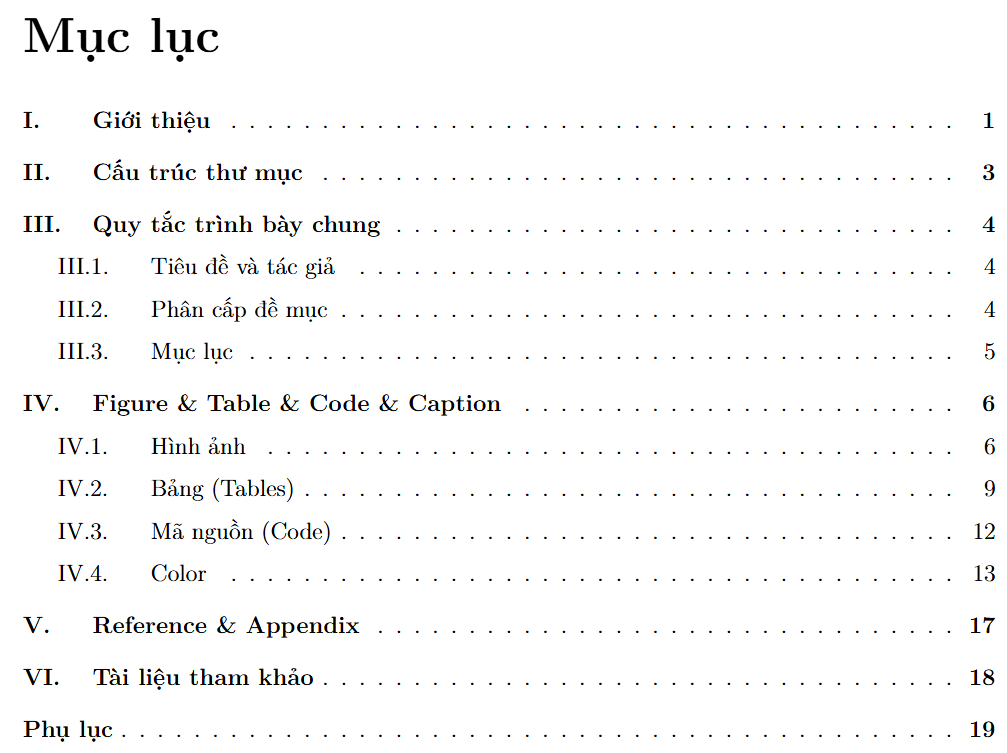
\includegraphics[width=0.8\linewidth]{Figures/table_of_contents.png}
    }
    \caption{Hình ảnh minh họa về cấu trúc mục lục}
\end{figure}

\newpage
\section{Các thành phần trực quan}

\subsection{Hình ảnh}

Hình ảnh trong tài liệu nên ưu tiên các định dạng như \textbf{.pdf} hoặc \textbf{.svg}, hoặc ít nhất phải bảo đảm văn bản bên trong hình có thể được quét và đọc rõ. Đây là yêu cầu quan trọng vì hình minh họa không chỉ có chức năng trang trí mà còn trực tiếp truyền đạt thông tin. Trong template này, phần caption cho hình có thể được trình bày theo nhiều cách khác nhau. 

\subsubsection{Kiểu 1: Mẫu truyền thống với \texttt{\textbackslash caption\{\}} đơn giản}

Người viết có thể dùng cách trình bày truyền thống của \LaTeX\ bằng môi trường \verb|figure| kết hợp với lệnh \verb|\caption|. Đây là lựa chọn phù hợp khi cần sự gọn nhẹ, quen thuộc, hoặc khi tài liệu phải tuân theo các chuẩn trình bày học thuật không dùng hộp màu.

\begin{aivnoutputbox}[Figure cơ bản với \texttt{\textbackslash caption}]
\begin{figure}[H]
    \centering
    \includegraphics[width=0.8\linewidth]{Figures/Search_Pipeline.pdf}
    \caption{Minh hoạ quy trình xử lý và phản hồi từ Llama3.1 với công cụ tìm kiếm. Với đường màu đỏ là phản hồi khi không sử dụng công cụ và ngược lại cho đường màu đen.}
    \label{fig:search_tool_2}
\end{figure}
\end{aivnoutputbox}

Kết quả hiển thị:

\begin{figure}[H]
    \centering
    \includegraphics[width=0.8\linewidth]{Figures/Search_Pipeline.pdf}
    \caption{Minh hoạ quy trình xử lý và phản hồi từ Llama3.1 với công cụ tìm kiếm. Với đường màu đỏ là phản hồi khi không sử dụng công cụ và ngược lại cho đường màu đen.}
    \label{fig:search_tool_2}
\end{figure}

Cách này đơn giản, dễ dùng, và đặc biệt phù hợp với các tài liệu theo chuẩn xuất bản như ACM hoặc IEEE, nơi caption thường được giữ ở dạng đơn sắc, không có nền hay viền trang trí.


\subsubsection{Kiểu 2: Caption ngắn, căn giữa, hộp màu chủ đề AI VIET NAM}

Với những hình minh họa quan trọng, đặc biệt là sơ đồ tổng quan hoặc block diagram, có thể dùng môi trường \verb|figurecardcaptionaivn| để tạo một hộp caption nổi bật với màu chủ đạo của template. Cách trình bày này giúp caption tách rõ khỏi phần hình, đồng thời tạo điểm nhấn thị giác ngay dưới minh họa.

\begin{center}
    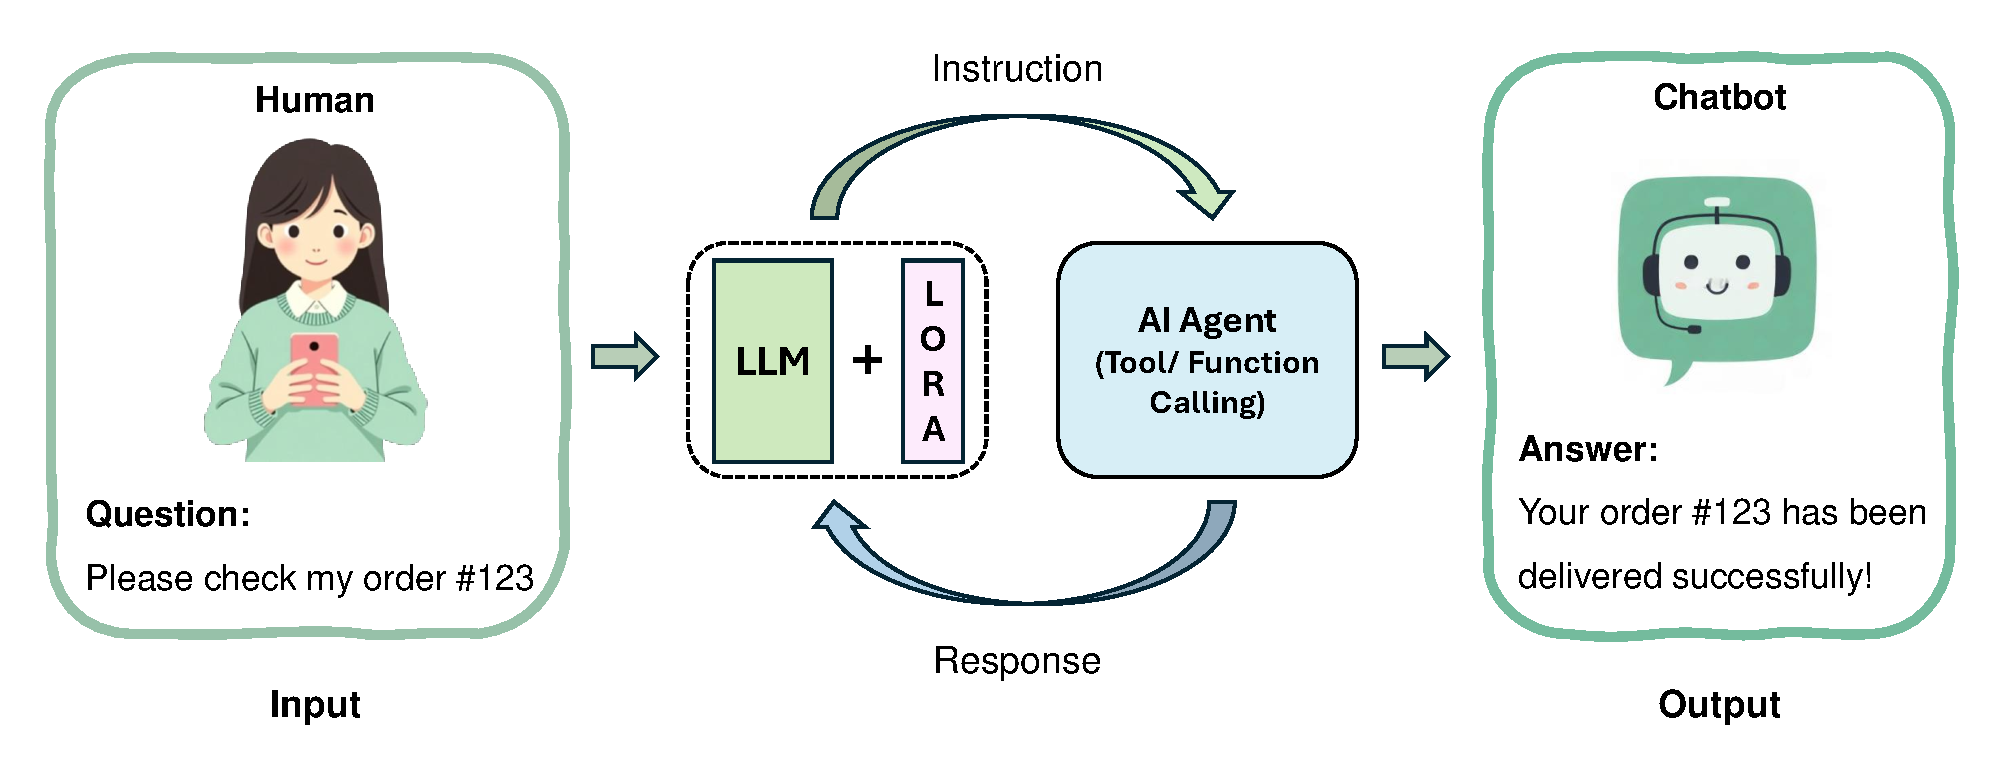
\includegraphics[width=\linewidth]{Figures/theme0.pdf}
    \begin{minipage}{0.75\linewidth}
    \begin{figurecardcaptionaivn}
    \centering
        \capfig{Minh họa bài toán QA sử dụng chatbot và AI Agent}
        \label{fig:toolcalling}
    \end{figurecardcaptionaivn}
    \end{minipage}
\end{center}

Trong ví dụ này, \verb|minipage| được dùng để giới hạn chiều rộng của box caption ở mức 75\% chiều rộng văn bản, nhờ đó caption không bị quá dài theo bề ngang. Bên trong box, lệnh \verb|\centering| giúp caption ngắn được căn giữa, còn lệnh \verb|\capfig{...}| sẽ tự động tăng bộ đếm hình và in ra số thứ tự tương ứng. Sau đó, \verb|\label{fig:toolcalling}| được dùng để tham chiếu trong nội dung tài liệu.

Kiểu này phù hợp khi hình có bố cục tương đối đơn giản, nền sáng, và caption ngắn. Hộp màu xanh đậm tạo độ tương phản rõ với nền trắng, nên rất hiệu quả với các hình cần được nhấn mạnh.

\subsubsection{Kiểu 3: Caption dài, căn trái, hộp viền màu trên nền sáng}

Không phải hình nào cũng phù hợp với một hộp caption có nền màu đậm. Với những hình đã chứa nhiều màu sắc hoặc chi tiết phức tạp, nên dùng môi trường \verb|figurecaptionmodern| để caption giữ phong cách tối giản hơn. Ở kiểu này, hộp caption có nền sáng và viền màu chủ đề, giúp phần chú thích vẫn đồng bộ với template nhưng không cạnh tranh thị giác với chính hình minh họa.

\begin{center}
    \includegraphics[width=0.8\linewidth]{Figures/Search_Pipeline.pdf}
    \begin{minipage}{0.85\linewidth}
    \begin{figurecaptionmodern}
     \raggedright
        \capfig{Minh hoạ quy trình xử lý và phản hồi từ Llama3.1 với công cụ tìm kiếm. Với đường màu đỏ là phản hồi khi không sử dụng công cụ và ngược lại cho đường màu đen.}
        \label{fig:search_tool}
    \end{figurecaptionmodern}
    \end{minipage}
\end{center}

Điểm phù hợp của kiểu này nằm ở chỗ nền box rất nhạt, gần với màu trắng, trong khi viền vẫn giữ màu \verb|aivnGreen| để không tách rời khỏi hệ màu chung. Với caption dài từ hai dòng trở lên, nên dùng \verb|\raggedright| để căn trái, giúp người đọc theo dõi nội dung dễ hơn thay vì để khối văn bản dài bị căn giữa.

Kiểu này nên dùng khi hình đã có nhiều màu sắc, khi cần một caption dài có tính diễn giải, hoặc khi muốn giảm bớt diện tích màu đậm trong bố cục tổng thể của trang.

\paragraph{Lưu ý khi chèn caption cho hình}

Khi trình bày hình ảnh, caption ngắn thường nên căn giữa để tạo cảm giác cân đối, còn caption dài nên căn trái để dễ đọc hơn.  Trong trường hợp dùng \verb|\caption| chuẩn của \LaTeX, nên đặt \verb|\label| sau \verb|\caption| để số hình và tham chiếu được liên kết đúng. Nhìn chung, người viết nên chọn kiểu caption sao cho phù hợp với chính đặc điểm của hình minh họa: hình càng nhiều chi tiết thì caption càng nên tiết chế; hình càng quan trọng thì caption càng nên rõ và dễ nhận diện.

\newpage
\subsection{Bảng}
\label{subsec:tables}

Bảng là thành phần dùng để tổ chức dữ liệu theo hàng và cột, giúp người đọc so sánh nhanh các giá trị, tiêu chí, hoặc kết quả thí nghiệm. Trong template này, bảng có thể được trình bày theo nhiều kiểu khác nhau, từ dạng cơ bản dùng \verb|\caption| mặc định của \LaTeX\ đến dạng có hộp chú thích theo phong cách nhận diện của AI VIET NAM. Việc chọn kiểu nào nên phụ thuộc vào độ phức tạp của nội dung, độ dài của caption, và mức độ nhấn mạnh mà người viết muốn tạo ra.

\subsubsection{Kiểu 1: Bảng cơ bản dùng \texttt{\textbackslash caption}}

Đây là cách trình bày đơn giản nhất. Người viết chỉ cần dùng môi trường \verb|table| kết hợp với \verb|\caption| và \verb|\label| như trong \LaTeX\ thông thường. Cách này phù hợp khi bảng ngắn, caption gọn, và không cần thêm hộp màu hay bố cục đặc biệt.

\begin{aivnoutputbox}[Bảng cơ bản với \texttt{\textbackslash caption}]
\begin{table}[H]
\centering
\caption{Evaluation results}
\label{tab:simple-caption}
\renewcommand{\arraystretch}{1.3}
\begin{tabularx}{0.9\linewidth}{@{}>{\centering\arraybackslash}X >{\centering\arraybackslash}X >{\centering\arraybackslash}X@{}}
  \toprule
  \textbf{Algorithm} & \textbf{Accuracy (\%)} & \textbf{Time (s)} \\
  \midrule
  Model A & 92.3 & 1.45 \\
  Model B & 89.7 & 1.32 \\
  Model C & 94.5 & 1.67 \\
  \bottomrule
\end{tabularx}
\end{table}
\end{aivnoutputbox}

Kết quả hiển thị:

\begin{table}[H]
\centering
\caption{Evaluation results}
\label{tab:simple-caption}
\renewcommand{\arraystretch}{1.3}
\begin{tabularx}{0.9\linewidth}{@{}>{\centering\arraybackslash}X >{\centering\arraybackslash}X >{\centering\arraybackslash}X@{}}
  \toprule
  \textbf{Algorithm} & \textbf{Accuracy (\%)} & \textbf{Time (s)} \\
  \midrule
  Model A & 92.3 & 1.45 \\
  Model B & 89.7 & 1.32 \\
  Model C & 94.5 & 1.67 \\
  \bottomrule
\end{tabularx}
\end{table}

Khi cần một cách làm nhanh, dễ hiểu, và bám sát cú pháp chuẩn của \LaTeX, đây là lựa chọn nên ưu tiên. Ngoài ra, vì \verb|\caption| tự xử lý đánh số và tham chiếu, người viết không cần tăng bộ đếm thủ công.

\subsubsection{Kiểu 2: Bảng có caption theo box của template}

Khi muốn bảng đồng bộ hơn với hệ nhận diện của AI VIET NAM, có thể dùng môi trường \verb|captionbelowboxaivn| đã được template định nghĩa sẵn. Kiểu này tạo một hộp caption riêng, giúp phần chú thích nổi bật hơn so với cách trình bày mặc định.

\begin{table}[H]
\centering
\begin{minipage}{0.9\linewidth}
  \refstepcounter{table}
  \begin{captionbelowboxaivn}
    Bảng~\thetable: Evaluation results
    \label{tab:box-caption}
  \end{captionbelowboxaivn}
  \renewcommand{\arraystretch}{1.3}
  \begin{tabularx}{\linewidth}{@{}>{\centering\arraybackslash}X >{\centering\arraybackslash}X >{\centering\arraybackslash}X@{}}
    \toprule
    \textbf{Algorithm} & \textbf{Accuracy (\%)} & \textbf{Time (s)} \\
    \midrule
    Model A & 92.3 & 1.45 \\
    Model B & 89.7 & 1.32 \\
    Model C & 94.5 & 1.67 \\
    \bottomrule
  \end{tabularx}
\end{minipage}
\end{table}

Kiểu này phù hợp khi caption ngắn, bảng không quá rộng, và người viết muốn giữ sự thống nhất với các box màu khác trong tài liệu.

\subsubsection{Kiểu 3: Bảng đi kèm đoạn văn mô tả song song}

Trong một số trường hợp, bảng cần được giải thích ngay tại chỗ thay vì để người đọc tự suy diễn từ caption. Khi đó, có thể đặt một đoạn mô tả song song với bảng trong cùng một khối trình bày. Cách này hữu ích khi bảng chỉ chiếm khoảng một nửa chiều ngang trang và phần diễn giải ngắn gọn nhưng quan trọng.

\begin{table}[H]
\centering
\begin{tabular}{@{}m{0.48\linewidth} m{0.47\linewidth}@{}}
  \justifying
  \noindent Bảng~\ref{tab:eval-parallel} trình bày kết quả đánh giá hiệu suất của ba mô hình dựa trên hai tiêu chí chính là độ chính xác và thời gian thực thi.
  &
  \begin{minipage}{\linewidth}
    \refstepcounter{table}
    \begin{captionbelowboxaivn}
      Bảng~\thetable: Evaluation results
      \label{tab:eval-parallel}
    \end{captionbelowboxaivn}
    \renewcommand{\arraystretch}{1.3}
    \begin{tabularx}{\linewidth}{@{}>{\centering\arraybackslash}X >{\centering\arraybackslash}X >{\centering\arraybackslash}X@{}}
      \toprule
      \textbf{Algo} & \textbf{Acc} & \textbf{Time} \\
      \midrule
      A & 92.3 & 1.45 \\
      B & 89.7 & 1.32 \\
      C & 94.5 & 1.67 \\
      \bottomrule
    \end{tabularx}
  \end{minipage}
\end{tabular}
\end{table}

Kiểu này nên dùng khi phần mô tả thực sự giúp người đọc hiểu bảng tốt hơn. Nếu lời giải thích dài, nên tách thành một đoạn độc lập trước hoặc sau bảng để bố cục không bị nặng.

\subsubsection{Kiểu 4: Header nhiều dòng}

Khi tiêu đề cột dài hoặc cần ghi song ngữ, có thể dùng \verb|\makecell| để tách header thành nhiều dòng. Cách này giúp bảng gọn hơn theo chiều ngang mà vẫn giữ nội dung rõ ràng.

\begin{table}[H]
\centering
\begin{minipage}{0.95\linewidth}
  \refstepcounter{table}
  \begin{captionbelowboxaivn}
    Bảng~\thetable: Accuracy and Latency of Models under Different Settings
  \end{captionbelowboxaivn}
  \renewcommand{\arraystretch}{1.4}
  \begin{tabularx}{\linewidth}{
    >{\centering\arraybackslash}p{0.35\linewidth}
    >{\centering\arraybackslash}p{0.25\linewidth}
    >{\centering\arraybackslash}p{0.25\linewidth}}
    \toprule
    \makecell{\textbf{Tên mô hình} \\ (Model Name)} &
    \makecell{\textbf{Độ chính xác} \\ (Accuracy \%)} &
    \makecell{\textbf{Thời gian thực thi} \\ (Time in s)} \\
    \midrule
    Llama3.1--v1 fine-tuned & 94.8 & 1.67 \\
    Phi-2 pretrained & 89.1 & 1.45 \\
    Qwen1.5--Chat--0.5B & 87.9 & 1.32 \\
    \bottomrule
  \end{tabularx}
\end{minipage}
\end{table}

Kiểu header nhiều dòng phù hợp với bảng có tên cột dài, nhiều chú giải, hoặc cần hiển thị cả tên tiếng Anh lẫn tiếng Việt.

\subsubsection{Kiểu 5: Bảng với caption dài}

Khi caption không chỉ là một tiêu đề ngắn mà còn mang tính diễn giải, nên căn trái để văn bản dễ đọc hơn. Trong trường hợp này, độ rộng của bảng và caption nên được kiểm soát bằng \verb|minipage| để toàn bộ khối giữ được sự cân đối.

\begin{table}[H]
\centering
\begin{minipage}{0.8\linewidth}
  \refstepcounter{table}
  \begin{captionbelowboxaivn}
    \raggedright
    Bảng~\thetable: Evaluation results across various model configurations showing accuracy and execution time metrics. The table illustrates model behavior under constrained latency settings, which is critical for applications requiring real-time responsiveness such as autonomous systems or interactive agents.
  \end{captionbelowboxaivn}
  \renewcommand{\arraystretch}{1.3}
  \begin{tabularx}{\linewidth}{@{}>{\centering\arraybackslash}X >{\centering\arraybackslash}X >{\centering\arraybackslash}X@{}}
    \toprule
    \textbf{Algo} & \textbf{Acc} & \textbf{Time} \\
    \midrule
    A & 92.3 & 1.45 \\
    B & 89.7 & 1.32 \\
    C & 94.5 & 1.67 \\
    \bottomrule
  \end{tabularx}
\end{minipage}
\end{table}

\paragraph{Lưu ý khi trình bày bảng}

Khi dùng \verb|\caption| mặc định, \LaTeX\ sẽ tự đánh số bảng và cho phép tham chiếu qua \verb|\label| mà không cần thao tác thêm. Ngược lại, khi dùng một box caption tự định nghĩa như \verb|captionbelowboxaivn|, người viết cần chủ động gọi \verb|\refstepcounter{table}| trước phần caption để tạo số bảng và hỗ trợ tham chiếu.

Về căn lề, caption ngắn có thể để ở dạng gọn và cân đối, trong khi caption dài nên căn trái bằng \verb|\raggedright| hoặc \verb|\justifying| để tránh cảm giác rời dòng. Với những bảng cần kiểm soát tốt độ rộng hoặc cần ghép cùng phần mô tả, nên đặt toàn bộ caption và bảng trong một \verb|minipage| để giữ chúng trong cùng một khối, tránh tình trạng caption và bảng bị tách sang hai trang khác nhau.


\newpage
\subsection{Mã nguồn}
\label{subsec:code}

Class file đã định nghĩa sẵn môi trường \verb|aivncodebox| để trình bày mã nguồn Python theo định dạng thống nhất. Môi trường này sử dụng \verb|tcolorbox| kết hợp với \verb|listings| để hiển thị mã trong một khung nổi bật, đồng thời giữ cách trình bày đồng bộ với toàn bộ template. Vì \verb|aivncodebox| được cấu hình với tùy chọn \verb|listing only|, người viết cần đặt mã trực tiếp vào bên trong box.

Nếu không muốn hiển thị tiêu đề, có thể để trống tham số tùy chọn. Ví dụ:

\begin{aivnoutputbox}[Box aivncodebox]
\begin{aivncodebox}[]
\begin{python}
def factorial(n):
    if n <= 1:
        return 1
    else:
        return n * factorial(n - 1)
print(factorial(5))
\end{python}
\end{aivncodebox}
\end{aivnoutputbox}

Kết quả hiển thị:

\begin{aivncodebox}[]
\begin{python}
def factorial(n):
    if n <= 1:
        return 1
    else:
        return n * factorial(n - 1)
print(factorial(5))
\end{python}
\end{aivncodebox}

Khi cần đặt tên cho đoạn mã, có thể truyền tiêu đề trong dấu ngoặc vuông. Cách này phù hợp với các đoạn mã có chức năng rõ ràng, chẳng hạn như một hàm, một thuật toán, hoặc một ví dụ minh họa cụ thể.

\begin{aivnoutputbox}[Box aivncodebox \texttt{\textbackslash caption}]
\begin{aivncodebox}[Hàm tính giai thừa]
\begin{python}
def factorial(n):
    if n <= 1:
        return 1
    else:
        return n * factorial(n - 1)

print(factorial(5))
\end{python}
\end{aivncodebox}
\end{aivnoutputbox}

\newpage
Kết quả hiển thị:

\begin{aivncodebox}[Hàm tính giai thừa]
\begin{python}
def factorial(n):
    if n <= 1:
        return 1
    else:
        return n * factorial(n - 1)
print(factorial(5))
\end{python}
\end{aivncodebox}

Khi trình bày mã nguồn, chỉ nên dùng tiêu đề khi đoạn mã thực sự cần được gọi tên để tiện
tham chiếu. Với các đoạn mã dài, nên tách thành nhiều khối theo từng chức năng để người đọc
dễ theo dõi. Trong hầu hết trường hợp, nên dán mã trực tiếp thay vì chụp ảnh màn hình, vì mã văn bản có thể sao chép, tìm kiếm, và tái sử dụng thuận tiện hơn.
\newpage
\subsection{Color}

Template đã định nghĩa sẵn hệ màu để người viết có thể mở rộng cách trình bày ngoài màu xanh mặc định của AI VIET NAM. Màu chủ đạo của template được khai báo như sau:

\begin{aivnoutputbox}[Khai báo màu chủ đạo]
\definecolor{aivnGreen}{RGB}{52,79,30}
\end{aivnoutputbox}

Các màu này có thể được đưa vào những tham số quen thuộc như \verb|colframe|, \verb|colbacktitle|, hoặc \verb|\rowcolors| để thay đổi giao diện của bảng biểu, khung chú thích, và khung mã nguồn mà vẫn giữ được tính thống nhất.

\paragraph{Ví dụ với bảng biểu}

Trong bảng biểu, có thể thay màu viền và màu nền tiêu đề bằng một màu \verb|...Accent|, đồng thời thay màu nền xen kẽ của các dòng bằng một màu \verb|...Row|. Ví dụ:

\begin{aivnoutputbox}[]
\begin{tcolorbox}[
  colframe=aivnGreen,      % có thể đổi thành màu khác, ...
  colbacktitle=aivnGreen,  % có thể đổi thành màu khác, ...
  colback=white,
  boxrule=1pt,
  title=\textbf{Bảng thuật ngữ},
  fonttitle=\bfseries\color{white},
  halign title=center,
  arc=5pt
]
\renewcommand{\arraystretch}{1.5}
\renewcommand{\tabularxcolumn}[1]{m{#1}}
\rowcolors{2}{white}{green!12!white}   % có thể đổi thành màu khác, ...
\begin{tabularx}{\linewidth}{>{\centering\arraybackslash}m{3.0cm} X}
...
\end{tabularx}
\end{tcolorbox}
\end{aivnoutputbox}

Kết quả minh họa:

\begin{tcolorbox}[
  colframe=aivnGreen,
  colbacktitle=aivnGreen,
  colback=white,
  boxrule=1pt,
  title=\textbf{Bảng thuật ngữ (aivnGreen \& green!12!white)},
  fonttitle=\bfseries\color{white},
  halign title=center,
  arc=5pt
]
\renewcommand{\arraystretch}{1.5}
\renewcommand{\tabularxcolumn}[1]{m{#1}}
\rowcolors{2}{white}{green!12!white}
\begin{tabularx}{\linewidth}{>{\centering\arraybackslash}m{3.0cm} X}
  \textbf{Thuật ngữ} & \textbf{Tạm dịch, ý nghĩa} \\
  \midrule
  Genetic Algorithm & \textbf{Giải thuật di truyền}: phương pháp tối ưu hoá theo quần thể, mô phỏng tiến hóa tự nhiên qua các bước chọn lọc, lai ghép và đột biến. \\
  Population & \textbf{Quần thể}: tập các cá thể ở một thế hệ. \\
  Individual & \textbf{Cá thể}: một lời giải ứng viên; trong One-Max là chuỗi nhị phân. \\
  Gene & \textbf{Gen}: cách biểu diễn của cá thể; trong One-Max là một bit 0/1. \\
\end{tabularx}
\end{tcolorbox}

\paragraph{Ví dụ với khung mã nguồn}

Tương tự, với khung mã nguồn, người viết chỉ cần thay các tham số màu trong phần định nghĩa box để tạo các biến thể khác nhau:

\begin{aivnoutputbox}
\newtcolorbox{aivncodebox}[1][]{
  enhanced,
  colback=gray!10,
  colframe={HTML}{333D91},      % có thể đổi thành màu khác, ...
  coltitle=white,
  colbacktitle={HTML}{EEECFA},  % có thể đổi thành màu khác, ...
  title=#1,
  ...
}
\end{aivnoutputbox}

Khi sử dụng hệ màu, nên giữ sự tiết chế để tài liệu không bị rời rạc về thị giác. Một cặp màu nên được dùng nhất quán trong cùng một nhóm thành phần, chẳng hạn cùng một loại bảng hoặc cùng một nhóm box minh họa. Cách này giúp tài liệu vừa có điểm nhấn, vừa giữ được bố cục ổn định và dễ theo dõi.

\newpage
\section{Tài liệu tham khảo \& Mục lục}

Phần cuối của tài liệu cần hoàn thiện hai thành phần: tài liệu tham khảo và phụ lục. Đây là phần giúp người đọc kiểm tra nguồn, lần lại các tài liệu đã sử dụng, và xem thêm những nội dung bổ trợ chưa đặt trong phần thân bài. Để quản lý danh mục tài liệu tham khảo một cách thống nhất, nên lưu toàn bộ thông tin trích dẫn trong file \texttt{references.bib}. Cách làm này giúp việc thêm, sửa, và tái sử dụng nguồn trở nên thuận tiện hơn, đồng thời giữ cho nội dung chính của tài liệu gọn và dễ kiểm soát.

\begin{aivnoutputbox}[]
\section{Tài liệu tham khảo}
\nocite{*}
\printbibliography
\end{aivnoutputbox}

Trong mẫu phía trên đây, lệnh \verb|\printbibliography| dùng để in danh mục tài liệu tham khảo, còn môi trường \verb|appendices| dùng để trình bày phần phụ lục. Nếu muốn hiển thị toàn bộ mục trong file \texttt{references.bib} thì có thể dùng \verb|\nocite{*}|; ngược lại, nếu chỉ muốn in những tài liệu đã được trích dẫn trong nội dung, có thể bỏ lệnh này đi. 

\begin{aivnoutputbox}[Mẫu về .bib tài liệu tham khảo]
\begin{appendices}
\begin{enumerate}
    \item \textbf{Datasets:} Các file dataset được đề cập trong bài có thể được tải tại \href{https://aivietnam.edu.vn/}{đây}.
\end{enumerate}
\end{appendices}
\end{aivnoutputbox}

Phần phụ lục nên chỉ chứa các nội dung thật sự cần thiết cho việc tra cứu thêm, chẳng hạn như liên kết dataset, mô tả cấu hình, biểu mẫu, hoặc tài liệu bổ sung.

\begin{aivnoutputbox}[Mẫu về phần phụ lục]
\begin{appendices}
\begin{enumerate}
    \item \textbf{AIVIETNAM:} Thông tin về AIVIETNAM có thể đọc thêm tại \href{https://aivietnam.edu.vn/}{đây}.
\end{enumerate}
\end{appendices}
\end{aivnoutputbox}

\newpage
\section{Tài liệu tham khảo}
\label{section:references}
\nocite{*}
\vspace{-3.2em}   
\printbibliography

\begin{appendices}
\begin{enumerate}
    \item \textbf{AIVIETNAM:} Thông tin về AIVIETNAM có thể đọc thêm tại \href{https://aivietnam.edu.vn/}{đây}.
\begin{figure}[H]
    \centering
    
\includegraphics[width=\textwidth]{Figures/AIO_QAs_Theme.jpg}
    \caption{Hình ảnh group facebook AIO Q\&A.}
    \label{fig:qa_theme}
\end{figure}
\end{enumerate}
\end{appendices}


\begin{center}
    Hết.
\end{center}
\end{document}
